\chapter{Decomposition Approach Evaluation}
\label{appendix:decompositionAppraoches}

During early feasibility tests with graph clustering, we encountered significant problems as documented in the next section. As consequence of these results, we conducted a feasibility assessment with a professor of mathematics on the graph based approach, documented in Appendix \ref{sec:feasibilityAssessment}. Out of the feasibility assessment, two additional approaches on how the Service Cutter can solve the decomposition problem were defined and are discussed in this chapter. Nevertheless, the conclusion section states how challenges in these approaches and further research on clustering graphs led us back to follow the graph based approach.

\section{Graph Clustering Problems}

At first, the clustering algorithm evaluated documented in Appendix \ref{appendix:graphClustering} did not contain the Leung algorithm as this has been found later during the project. The two candidate algorithms were MCL and Girvan-Newman. We did a feasibility test using a small booking sample containing three entities:

\begin{description}
	\item[Customer Entity] containing address, accountNr, creditCardNr, and name.
	\item[Article Entity] containing articleName, price, and serial.
	\item[Booking Entity] containing totalPrice, paymentDate, bookingDate, and bookingState.
\end{description}

\begin{figure}[H]
	\begin{center}
		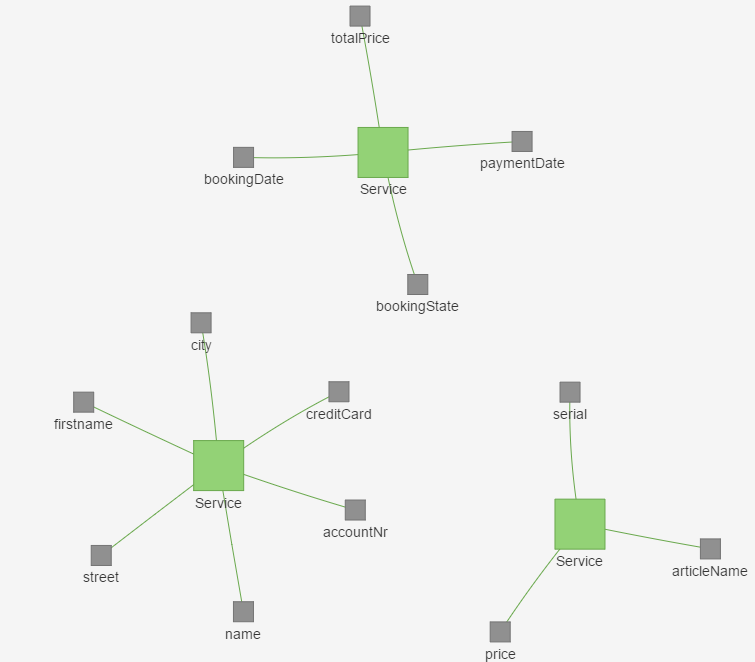
\includegraphics[scale=0.75]{images/booking_entities.png}
	\end{center}
	\caption{Expected output for the booking example.}
	\label{fig:bookingExample}
\end{figure}

To keep the sample simple we only added information for the \textit{Lifecycle \& Identity Commonality} criterion, so that the output is expected to show exactly the entity borders as shown in Figure \ref{fig:bookingExample}.


\begin{figure}[H]
	\begin{center}
		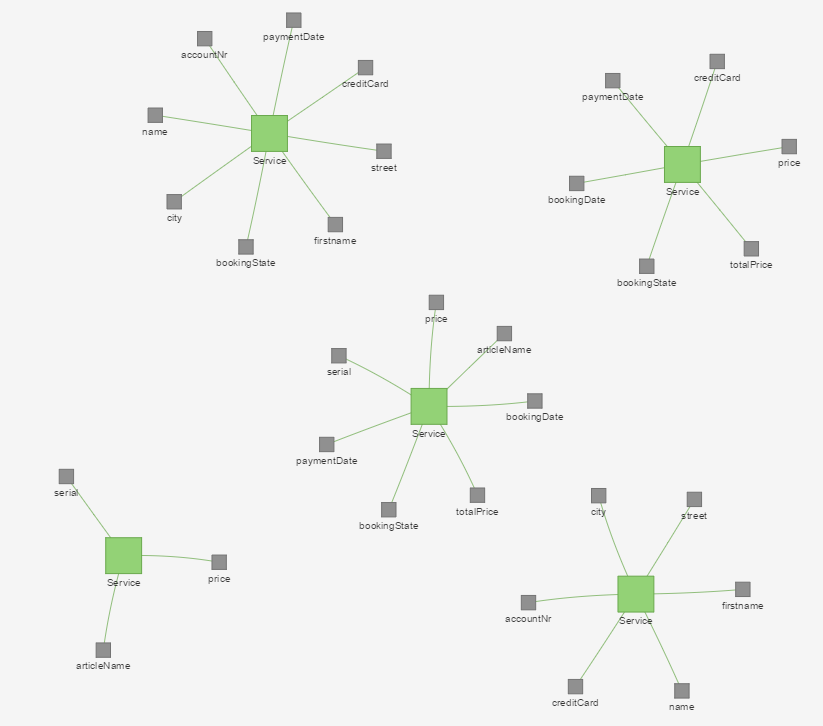
\includegraphics[scale=0.7]{images/booking_entities_mcl.png}
	\end{center}
	\caption{booking sample with the MCL algorithm.}
	\label{fig:bookingExampleMCL}
\end{figure}

The MCL algorithm's result for this example is shown in Figure \ref{fig:bookingExampleMCL}. This does not match the expectations as nanoentities are attached to multiple services. This violates the \textit{distinct clusters} requirement. A nanoentity should be assigned to one and only one service. 

The distinct clusters requirement is satisfied by the original MCL algorithm written in C. We therefore assume that this is  an implementation problem of the Gephi plugin\cite{gephiMarkov}. A solution to this problem would be to write a Java wrapper for the C implementation as described in Section \ref{subsec:mclAdapter}.

\begin{figure}[H]
	\begin{center}
		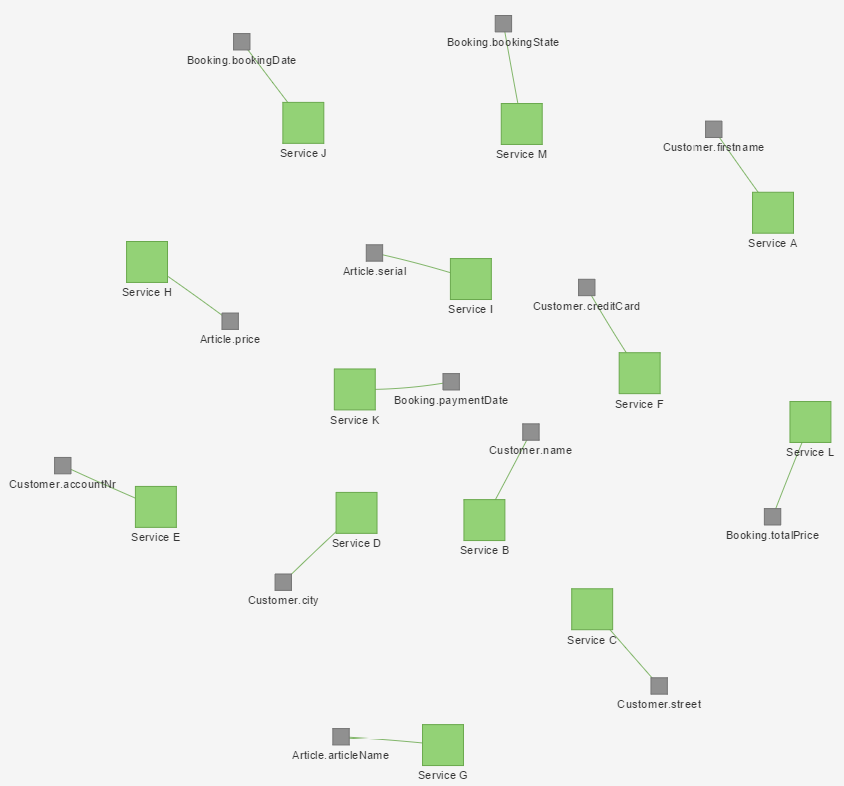
\includegraphics[scale=0.65]{images/girvan_entities_fail.png}
	\end{center}
	\caption{Booking example with the Girvan-Newman algorithm.}
	\label{fig:bookingExampleGirvan}
\end{figure}

Figure \ref{fig:bookingExampleGirvan} shows the unsatisfying result provided by Girvan-Newman. By reasons of these unexpected results, we consulted a professor of mathematics as documented in Appendix \ref{sec:feasibilityAssessment} which lead to the alternative approaches described in the next Sections.

\section{Approach \#2: Rating of Possible Service Cuts}

The idea this approach introduces is to create a set of all possible service cuts and rate the cuts isolated per coupling criteria. The approach is illustrated in Figure \ref{fig:setProcess}.


\begin{figure}[H]
	\begin{center}
		\includegraphics[scale=0.45]{diagrams/scoring_process.png}
	\end{center}
	\caption{Approach \#2: Service Cut Rating}
	\label{fig:setProcess}
\end{figure}

This approach is processed in three steps:

\begin{description}
	\item[Partitioning] Based on the nanoentities, a set of all possible candidate service cuts is calculated. This includes every theoretically possible service cut for any number of services. For practical usage, this step needs to be optimized. 
	\item[Assessment] For all coupling criteria a processor assesses all service cuts with a score describing how well the criteria's requirements are met. The score is a number between 0 and 10, while 10 implies that all requirements are perfectly satisfied. 
	\item[Evaluation] The user optionally defines priorities how important each criteria is for his system. The priorities are defined with approximately exponential numbers like the Fibonacci sequence. These priorities are applied on the service cut scores. The resulting best candidate cut is then presented to the user.
\end{description}

\subsection{Discussion}

An advantage of this approach is that each relevant step is clearly separated and can thus be analyzed, debugged and visualized better than in the graph based approach. The assessment and score calculation is done separately for every cut and for every coupling criteria. Each criteria scorer scores candidate cuts with a uniform scoring range. As candidate service cuts do not need to be constructed but only rated, the single dimensionality problem described in Section \ref{subsec:singleDimensionality} does not apply.

The weak spot is the partitioning process. Theoretically every possible set of services where each nanoentity is contained in one and only one service is a candidate cut. In mathematics this is described as the \textit{partition of a set}\cite{partitionOfASet} problem. The Bell number $B_n$ defines the amount of possible partitions: 


\begin{displaymath}
B_{n+1}=\sum_{j=0}^n {n\choose j} B_j
\end{displaymath}

For the Service Cutter, $n$ is the number of nanoentities. The number of possible service cuts for $n=20$ nanoentities is $51'724'158'235'372$\footnote{We do not print the number for the required $2000$ nanoentities for lack of space in this document.}.

The Bell number includes cuts for $1 - n$ number of services. In the context of a software system only certain numbers of services are realistic. The \textit{Stirling numbers of the second kind} calculate the Bell number for a given number of sets $k$:

\begin{displaymath}
\left\{ {n \atop k}\right\} = \frac{1}{k!}\sum_{j=0}^{k} (-1)^{k-j} \binom{k}{j} j^n
\end{displaymath}

For $n=20$ nanoentities and $k=4$ services the equation results in $45'232'115'901$ possible cuts. For $k=6$ the result is $4'306'078'895'384$.

During a discussion with our industry partner and supervisor documented in Appendix \ref{sec:status22102015}, we decided that the Service Cutter should be able to process system models with up to 2000 nanoentities. We therefore concluded in the same meeting that this approach is not attainable without a heuristic attempt of finding a small set of relevant candidate cuts. 

A possible heuristic approach is to take into account one or a few coupling criteria information about the system to find service candidates. A simple example would be to only analyze cuts where nanoentities of the same entity are not split across services so that only entities and not its nanoentities need to be considered.

As we tried to find a heuristic approach to calculate candidate cuts, we discovered a new idea for the composition algorithm described in the next section. 

\section{Approach \#3: Greedy Service Construction}

While analyzing the decomposition problem we realized that finding a good number of services is one of the key challenges. Cohesiveness criteria are mainly satisfied by consolidating nanoentities in one service while compatibility criteria request exactly the opposite, namely the separation of nanoentities. Figure \ref{fig:numberOfServices} illustrates this dilemma.

\begin{figure}[H]
	\begin{center}
		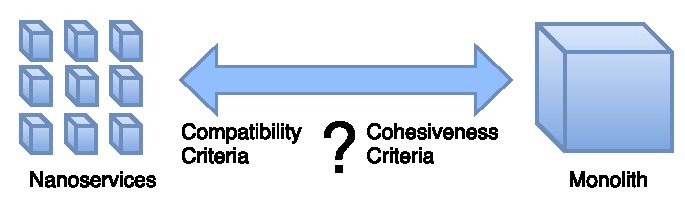
\includegraphics[scale=1]{diagrams/HeuristicApproach.pdf}
	\end{center}
	\caption{Finding a good number of services is a key challenge of service decomposition}
	\label{fig:numberOfServices}
\end{figure}

To simplify the problem we assume the number of services is given by the user and does not need to be computed. Very often an architect has a reasonable assumption about the number of services suitable for his system. 

Given the number of services, the services can be imagined as empty boxes that need to be filled with nanoentities. The boxes are filled by construction and optimization steps. In every construction step, one nanoentity is assigned to a box by means of a greedy algorithm.

\begin{description}
	\item[Construction Step] One nanoentity is taken from an unordered list of all unassigned nanoentities and put in the best suitable service. The suitability is calculated by the criteria scores between the selected nanoentity and the nanoentities already assigned to a service. 
\end{description}

Such greedy algorithms often end in a local maxima and not in the global maxima that represents the optimal solution. In every step the assignment decision is only based on the already assigned nanoentities. Assignments by former steps cannot be changed. 
To improve this behavior, the algorithm should process optimization steps between or after construction. 

\begin{description}
\item[Optimization Step] One service with already assigned nanoentities is randomly chosen. Within the service, the score from each nanoentity to all its neighbors is calculated to determine the least suitable nanoentity in a service. This nanoentity is taken out of the service and put back on the list of unassigned nanoentities.
\end{description}


The algorithm starts by assigning the first nanoentity to a random service and then alternates between construction and optimization stages. It finishes either after a given time, by the user stopping the optimization or by detecting that no further optimization is possible. This is detected when nanoentities taken from services in an optimization step are put back to their original service during the construction step. To finish the algorithm all nanoentities must be assigned to a service.

We have not proved that this algorithm solves the desired problem. The approach focuses only on cohesion within services but does not take coupling between services into consideration. Whether these two requirements build a duality, meaning that optimizing one automatically optimizes the other, is to be analyzed. However, we did not continue to investigate in this approach due to new findings on graph clustering described in the next section.

\subsection{New Findings on Graph Clustering}

Parallel to finding new approaches we continued to investigate the graph clustering.

By analyzing the Girvan-Newman algorithm documented in Section \ref{subsec:girvanNewman}, we were able to identify the problem encountered with the booking sample. As the sample only provides \textit{Lifecycle \& Identity Commonality} data, every pair of nanoentities in the graph was either directly or not connected at all. The calculated edge betweenness, which Girvan-Newman is based on, is therefore equal for all edges in the graph as every shortest path only passes one edge. The Gephi\cite{gephi} implementation of Girvan-Newman then consequently removes all edges in the first iteration leaving every nanoentity isolated which then results in one service per nanoentity. Adding only one more information like nanoentity characteristics or use cases solved this problem.

Through further research on the topic we found the algorithm defined by Leung implemented in the GraphStream\cite{leungGraphstream} project and integrated it into the Service Cutter. First tests using the booking sample provided the expected results.

\section{Conclusion}

While all approaches possibly lead to the desired results, the new findings on the Girvan-Newman and Leung algorithms promised the best results with adequate effort. Rating possible service cuts or heuristic construction of services would both require greater effort. Together with our stakeholders we decided that the effort is not worth taking, considering that the graph clustering provides reasonable results. 

We furthermore implemented a warning in the Service Cutter should a user provide input leading to the faulty behavior of Girvan-Newman as shown in Figure \ref{fig:girvanNewmanWarning}

\begin{figure}[H]
	\begin{center}
		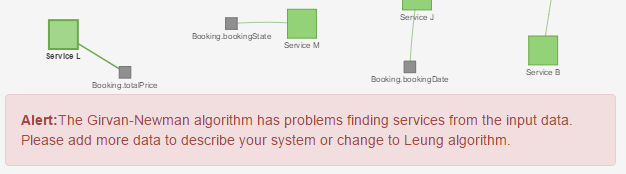
\includegraphics[scale=0.9]{images/grivanNewmanAlert.png}
	\end{center}
	\caption{Service Cutter shows a warning for faulty Girvan-Newman results.}
	\label{fig:girvanNewmanWarning}
\end{figure}
	